\chapter{Parameter patterns}
\label{appendix:patterns}
\begin{figure}[H]
	\centering
	\begin{subfigure}[t]{0.7\textwidth}
		\centering
		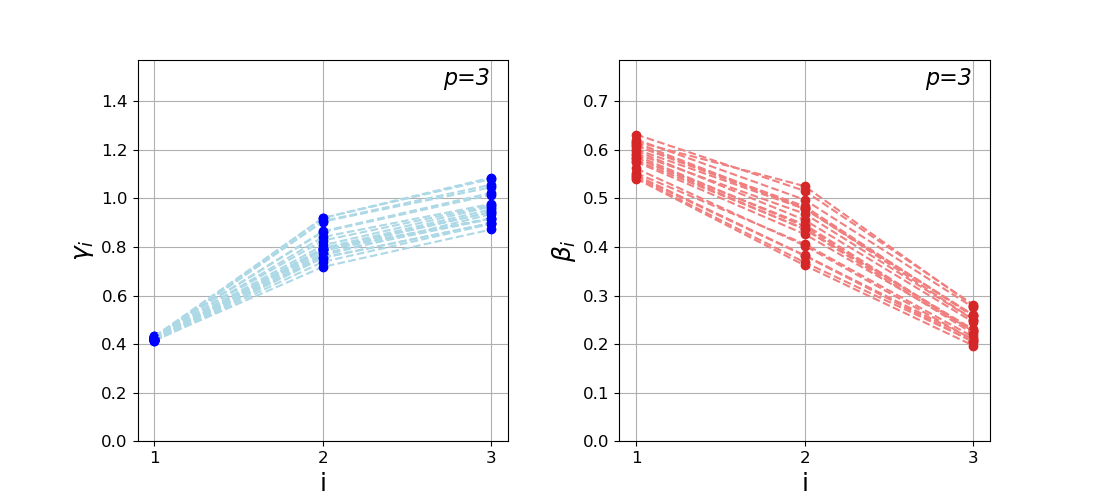
\includegraphics[width=\textwidth]{figures/interp/patterns/pattern_16-nodal_p-3.png}
	\end{subfigure}
	\\
	\centering
	\begin{subfigure}[t]{0.7\textwidth}
		\centering
		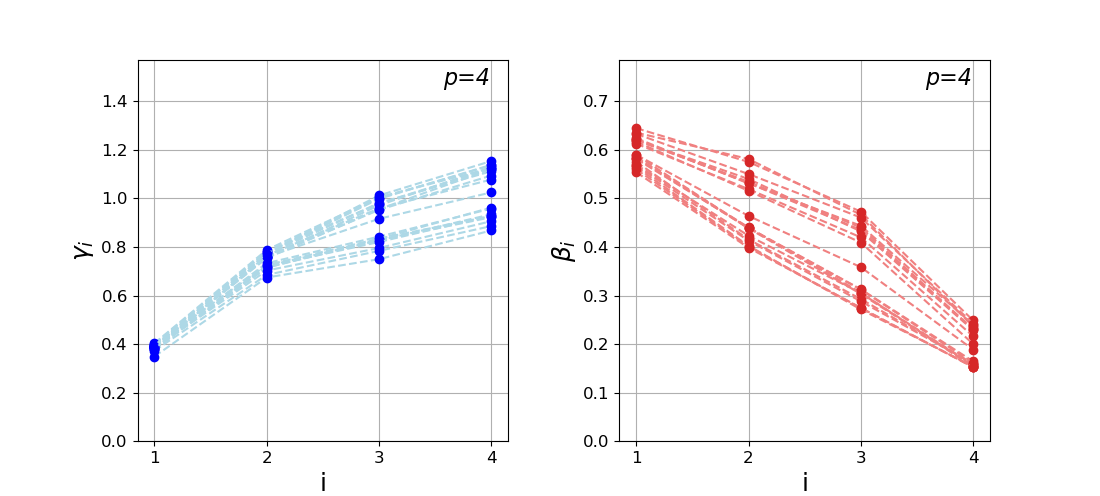
\includegraphics[width=\textwidth]{figures/interp/patterns/pattern_16-nodal_p-4.png}
	\end{subfigure}
	\\
	\centering
	\begin{subfigure}[t]{0.7\textwidth}
		\centering
		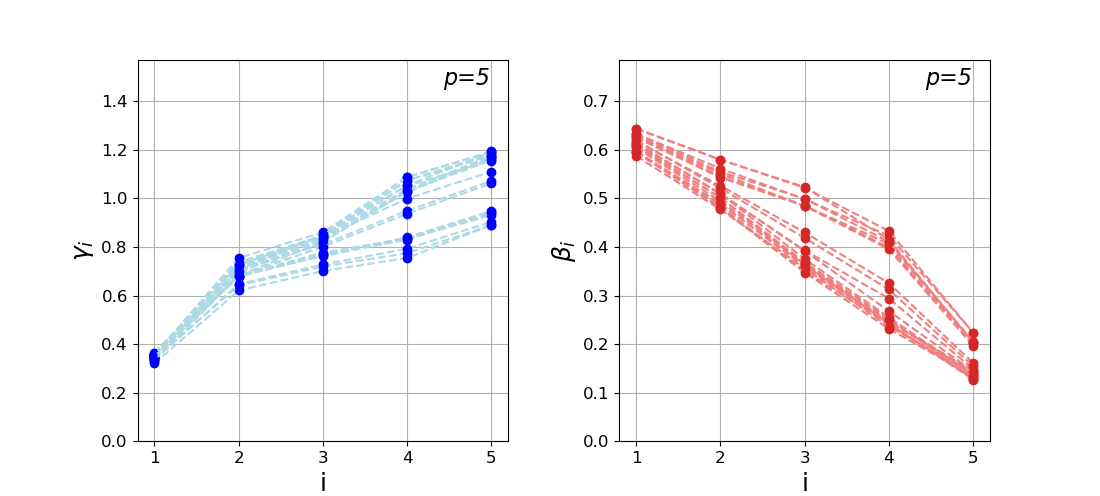
\includegraphics[width=\textwidth]{figures/interp/patterns/pattern_16-nodal_p-5.png}
	\end{subfigure}
	\caption{Quasi-optimal parameters $(\gambe)$ found using the pyQuil INTERP method for 20 instances of 3-regular unweighted graphs with 16 nodes for $p = 3, 4, 5$.}
	\label{fig:appendix-patterns-16-nodal}
\end{figure}

\newpage
\begin{figure}[H]
	\centering
	\begin{subfigure}[t]{0.7\textwidth}
		\centering
		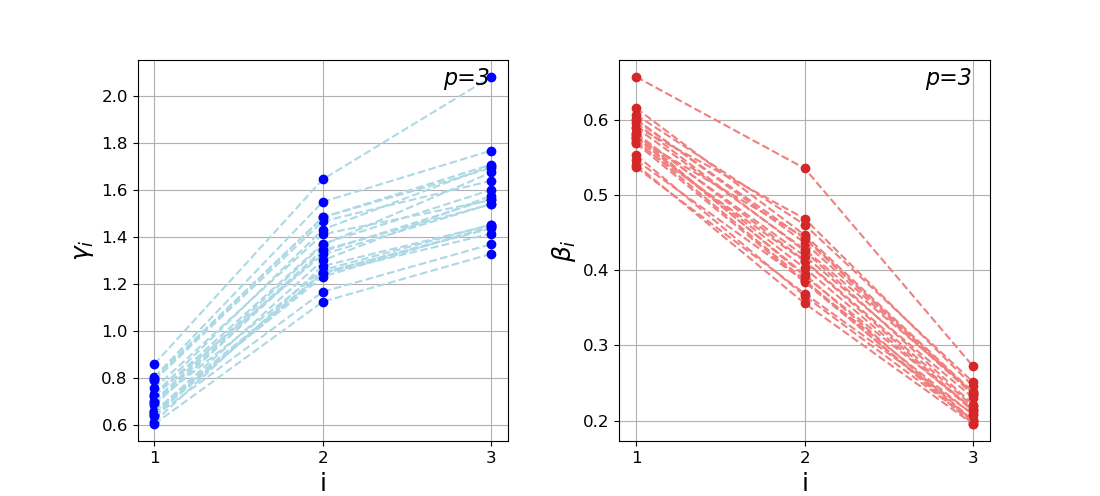
\includegraphics[width=\textwidth]{figures/interp/patterns/pattern_16-nodal_p-3_weighted.png}
	\end{subfigure}
	\\
	\centering
	\begin{subfigure}[t]{0.7\textwidth}
		\centering
		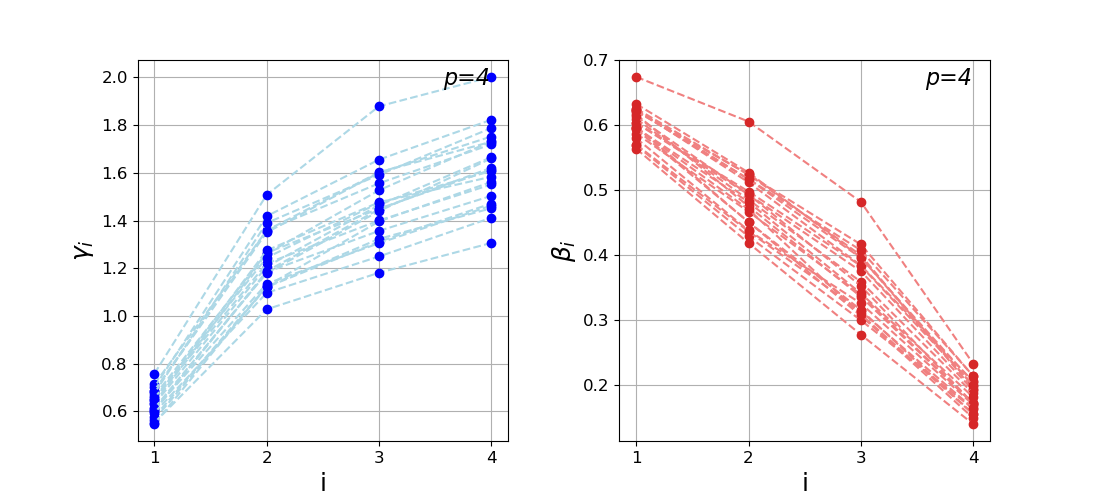
\includegraphics[width=\textwidth]{figures/interp/patterns/pattern_16-nodal_p-4_weighted.png}
	\end{subfigure}
	\\
	\centering
	\begin{subfigure}[t]{0.7\textwidth}
		\centering
		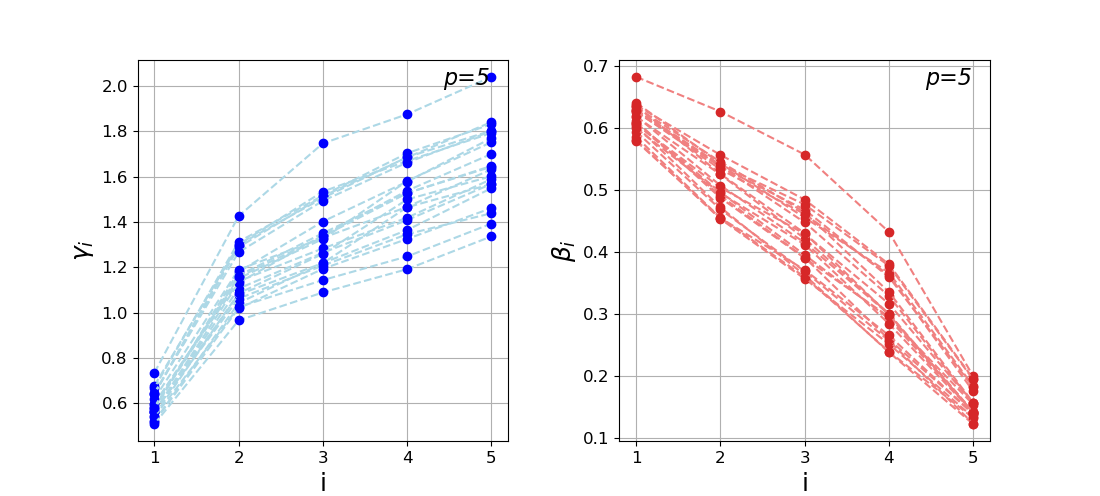
\includegraphics[width=\textwidth]{figures/interp/patterns/pattern_16-nodal_p-5_weighted.png}
	\end{subfigure}
	\\
	\centering
	\begin{subfigure}[t]{0.7\textwidth}
		\centering
		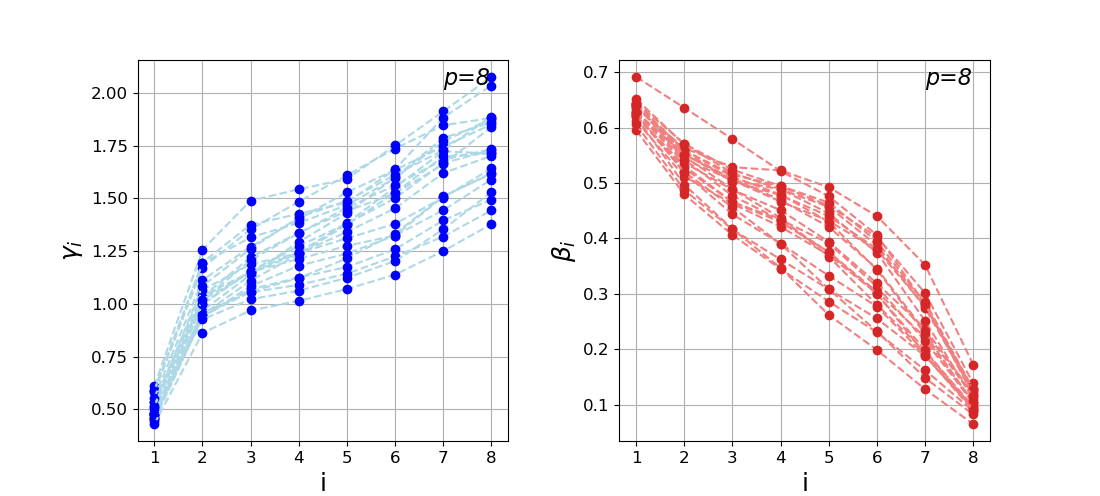
\includegraphics[width=\textwidth]{figures/interp/patterns/pattern_16-nodal_p-8_weighted.png}
	\end{subfigure}
	\caption{Quasi-optimal parameters $(\gambe)$ found using the pyQuil INTERP method for 20 instances of 3-regular weighted graphs with 16 nodes for $p = 3, 4, 5$ and $8$}
	\label{fig:appendix-patterns-12-nodal-3-regular}
\end{figure}

\newpage
\begin{figure}[H]
	\centering
	\begin{subfigure}[t]{0.7\textwidth}
		\centering
		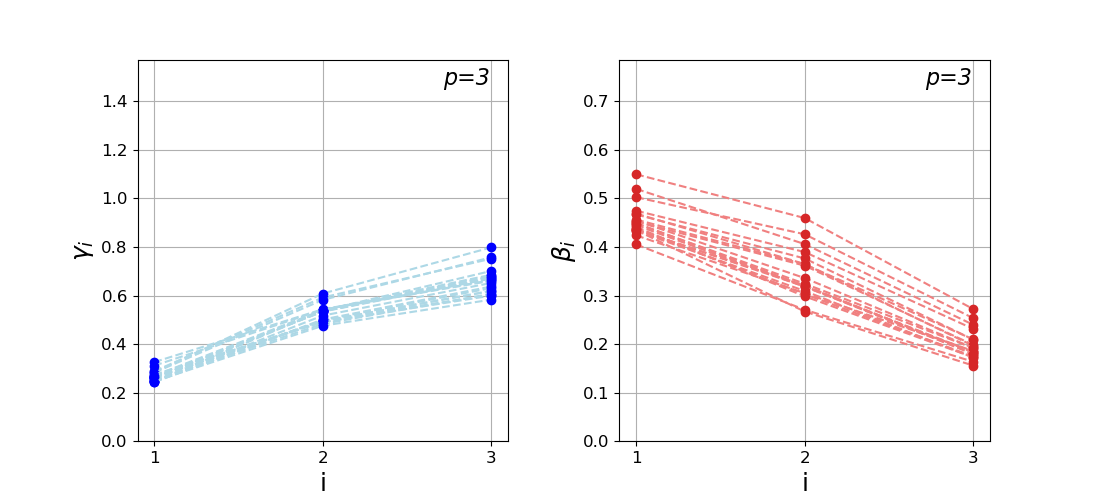
\includegraphics[width=\textwidth]{figures/interp/patterns/pattern_12-nodal_ER050_p-3.png}
	\end{subfigure}
	\\
	\centering
	\begin{subfigure}[t]{0.7\textwidth}
		\centering
		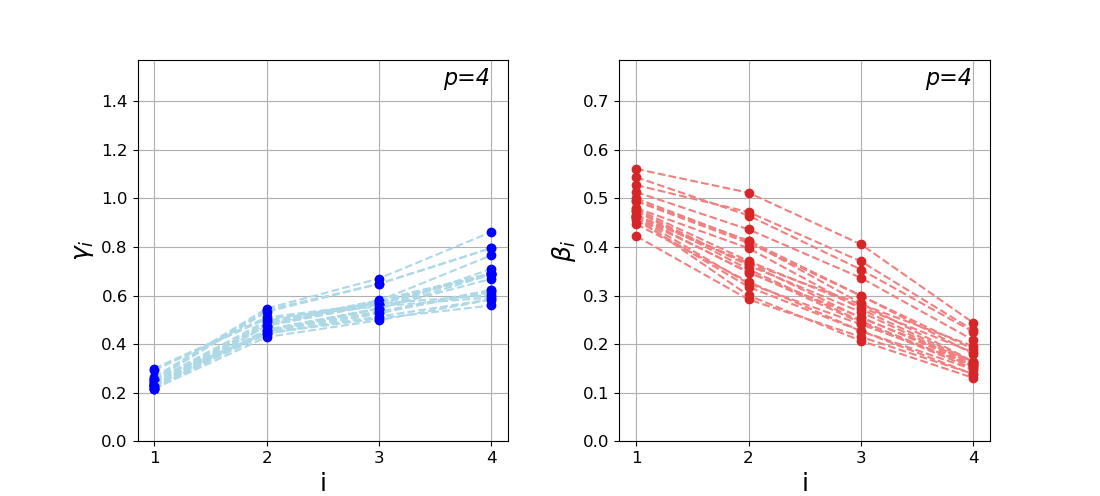
\includegraphics[width=\textwidth]{figures/interp/patterns/pattern_12-nodal_ER050_p-4.png}
	\end{subfigure}
	\\
	\centering
	\begin{subfigure}[t]{0.7\textwidth}
		\centering
		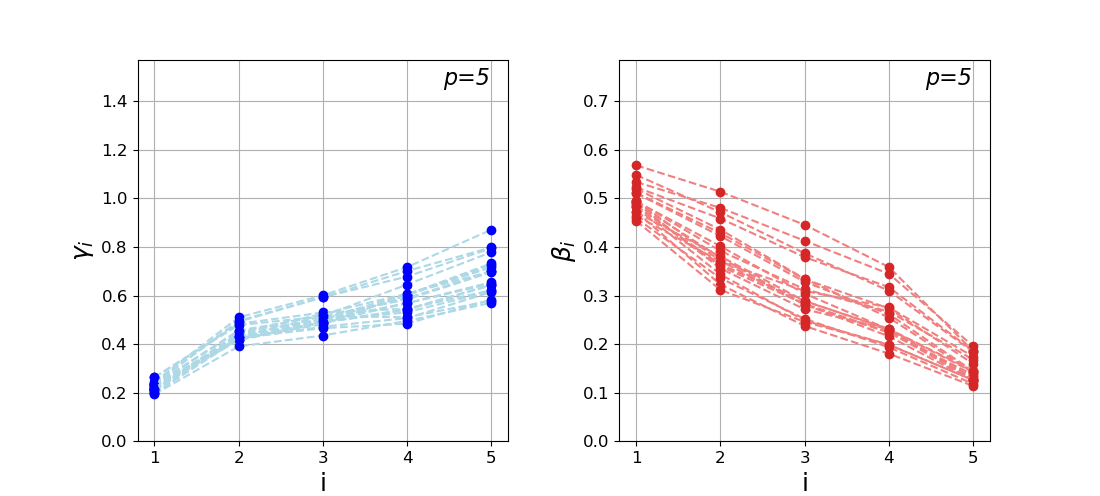
\includegraphics[width=\textwidth]{figures/interp/patterns/pattern_12-nodal_ER050_p-5.png}
	\end{subfigure}
	\\
	\centering
	\begin{subfigure}[t]{0.7\textwidth}
		\centering
		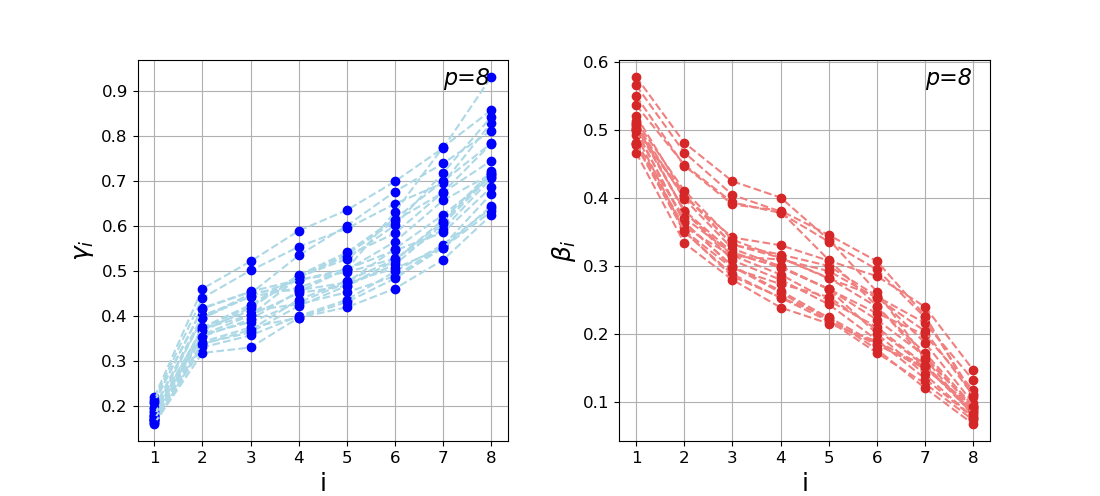
\includegraphics[width=\textwidth]{figures/interp/patterns/pattern_12-nodal_ER050_p-8.png}
	\end{subfigure}
	\caption{Quasi-optimal parameters $(\gambe)$ found using the pyQuil INTERP method for 20 instances of 12-nodal unweighted graphs drawn from the Erd\H{o}s-R\'enyi ensemble with edge probability 0.5 for $p = 3, 4, 5$ and $8$.}
	\label{fig:appendix-patterns-12-nodal-ER050}
\end{figure}

\newpage
\begin{figure}[H]
	\centering
	\begin{subfigure}[t]{0.7\textwidth}
		\centering
		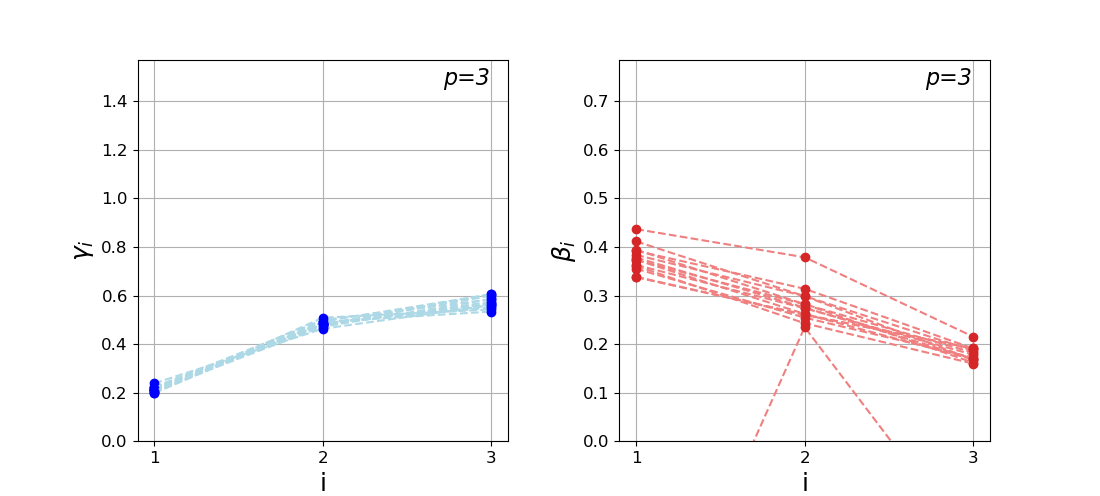
\includegraphics[width=\textwidth]{figures/interp/patterns/pattern_12-nodal_ER075_p-3.png}
	\end{subfigure}
	\\
	\centering
	\begin{subfigure}[t]{0.7\textwidth}
		\centering
		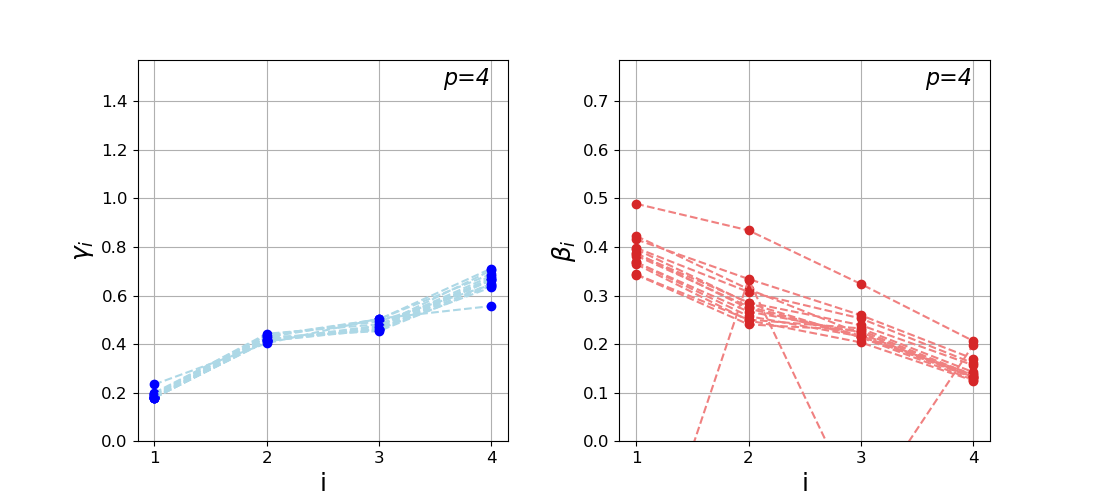
\includegraphics[width=\textwidth]{figures/interp/patterns/pattern_12-nodal_ER075_p-4.png}
	\end{subfigure}
	\\
	\centering
	\begin{subfigure}[t]{0.7\textwidth}
		\centering
		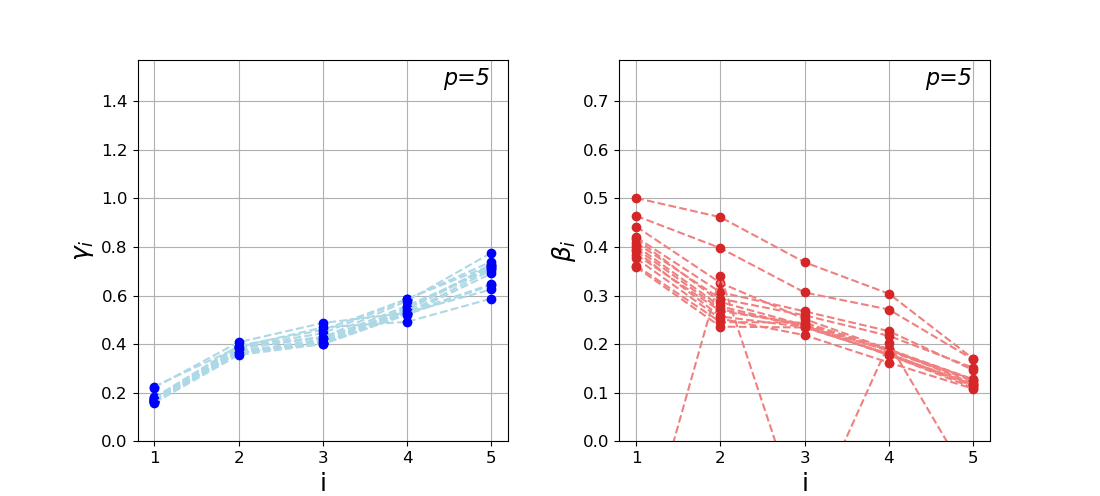
\includegraphics[width=\textwidth]{figures/interp/patterns/pattern_12-nodal_ER075_p-5.png}
	\end{subfigure}
	\\
	\centering
	\begin{subfigure}[t]{0.7\textwidth}
		\centering
		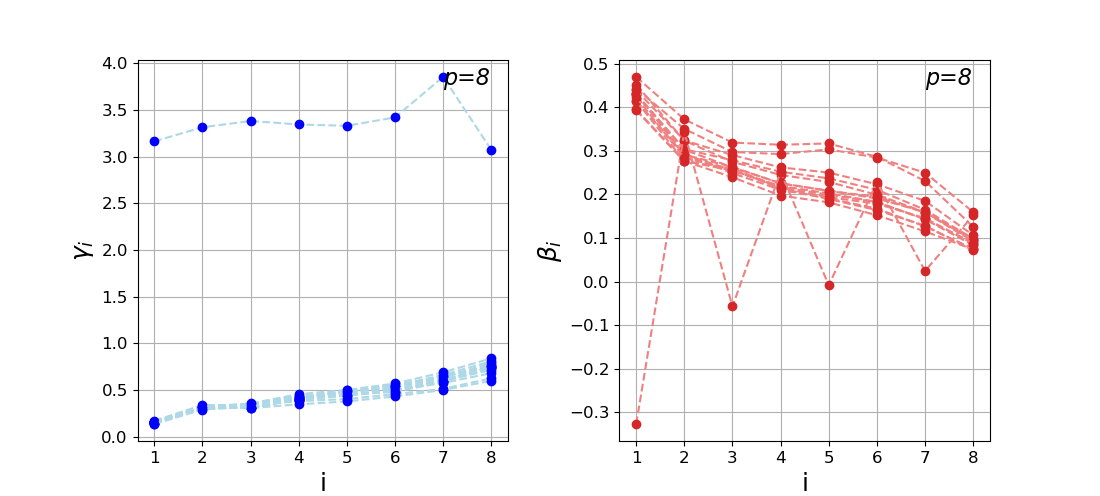
\includegraphics[width=\textwidth]{figures/interp/patterns/pattern_12-nodal_ER075_p-8.png}
	\end{subfigure}
	\caption{Quasi-optimal parameters $(\gambe)$ found using the pyQuil INTERP method for 10 instances of 12-nodal unweighted graphs drawn from the Erd\H{o}s-R\'enyi ensemble with edge probability 0.75 for $p = 3, 4, 5$ and 8. There seems to be one graph with anomalous results for which the $\beta_i$ parameter  oscillates around 0 and the $\gamma_i$ parameters lie around $\pi$. This is best seen on the graph for $p=8$, where I did not restict the limits of the vertical axis. Possibly this anomaly has to do with the degeneracy of the optima, as I only removed the degeneracies due to time-reversal symmetry.}
	\label{fig:appendix-patterns-12-nodal-ER075}
\end{figure}

\newpage
\begin{figure}[H]
	\centering
	\begin{subfigure}[t]{0.7\textwidth}
		\centering
		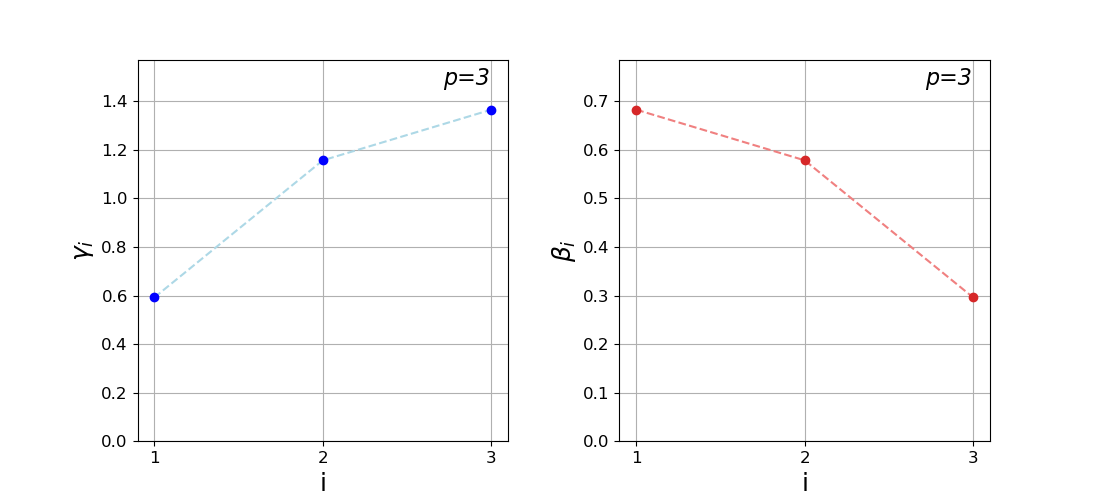
\includegraphics[width=\textwidth]{figures/interp/patterns/pattern_12-nodal_cyclic_p-3.png}
	\end{subfigure}
	\\
	\centering
	\begin{subfigure}[t]{0.7\textwidth}
		\centering
		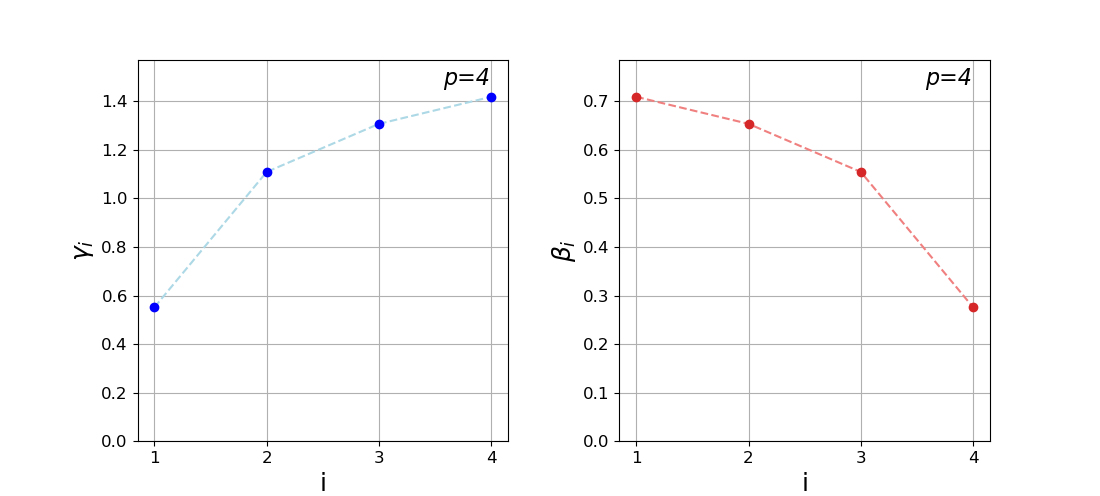
\includegraphics[width=\textwidth]{figures/interp/patterns/pattern_12-nodal_cyclic_p-4.png}
	\end{subfigure}
	\\
	\centering
	\begin{subfigure}[t]{0.7\textwidth}
		\centering
		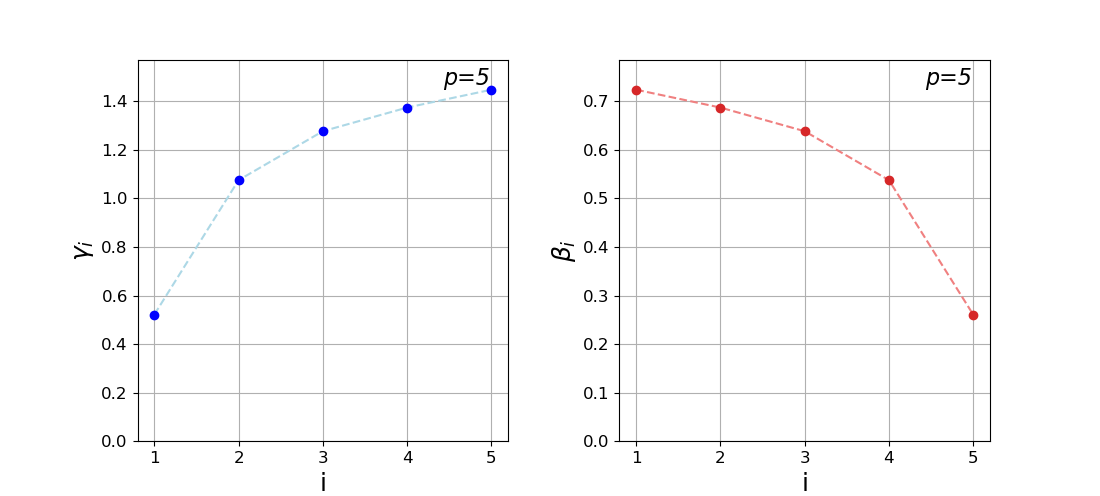
\includegraphics[width=\textwidth]{figures/interp/patterns/pattern_12-nodal_cyclic_p-5.png}
	\end{subfigure}
	\\
	\centering
	\begin{subfigure}[t]{0.7\textwidth}
		\centering
		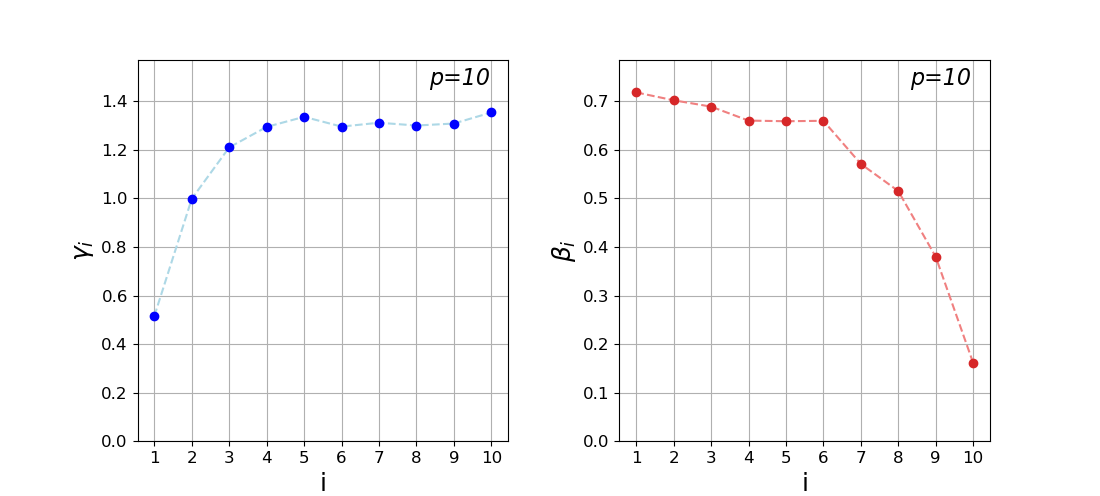
\includegraphics[width=\textwidth]{figures/interp/patterns/pattern_12-nodal_cyclic_p-10.png}
	\end{subfigure}
	\caption{Quasi-optimal parameters $(\gambe)$ found using the pyQuil INTERP method for the cyclic graph of 12 nodes for $p=3,4,5$ and $10$.}
	\label{fig:appendix-patterns-12-nodal-cyclic}
\end{figure}

\chapter{Runtime}
\label{appendix:runtime}
\begin{figure}[H]
	\centering
	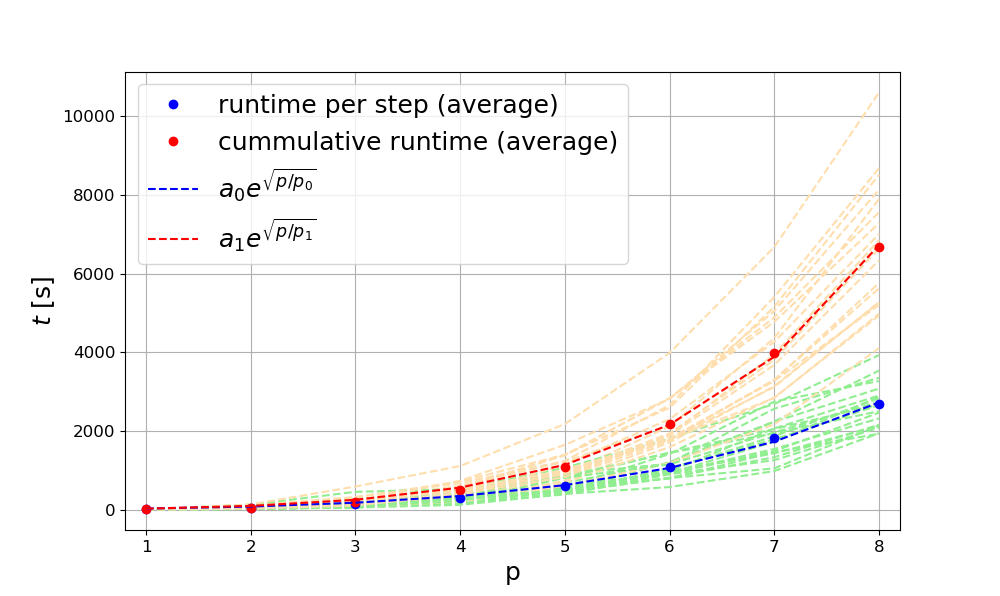
\includegraphics[width=0.6\textwidth]{figures/interp/runtime_16-nodal.png}
	\caption{Runtime (wall-clock time) when simulating the algorithm using the pyQuil INTERP method on 20 instances of 3-regular graph with 16 nodes. The fit parameters for the runtime per step are $a_0 = 2.4 \pm 0.6$, $p_0 = 6.1 \pm 0.4$. The fit parameters for the cummulative runtime are $a_1 = 1.4\pm 0.2$ and $p_1 = 9.0\pm0.3$. The mean runtime per graph per step at $p=8$ is around 2700 seconds, or 45 minutes. A run for one graph starting from $p=1$ typically lasted 2 hours. The light green and navajo white dashed lines indicate the runtime per step and the cummulative time for one instance, respectively.}
\end{figure}

\begin{figure}[H]
	\centering
	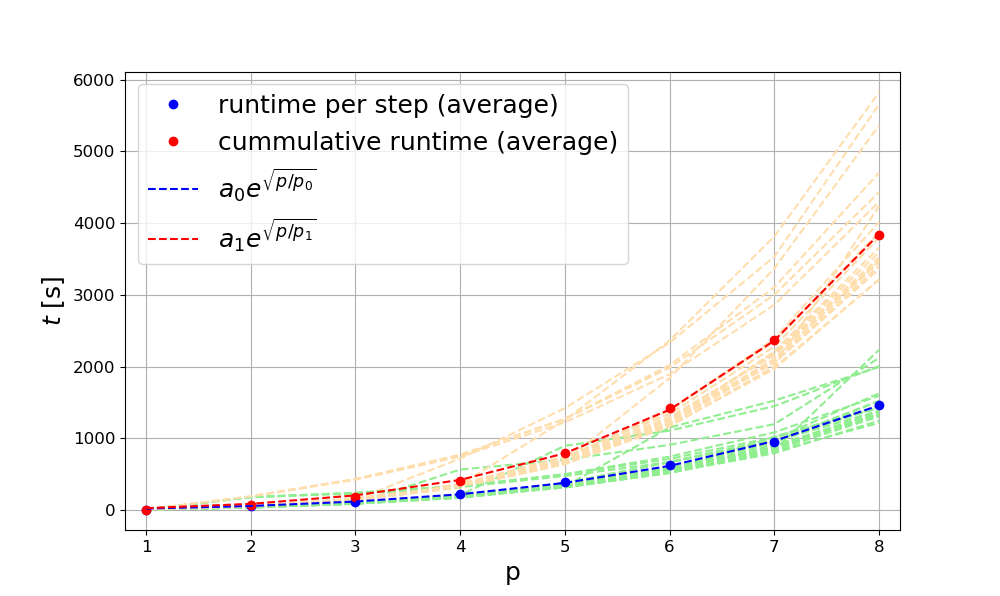
\includegraphics[width=0.6\textwidth]{figures/interp/runtime_16-nodal_weighted.png}
	\caption{Runtime (wall-clock time) when simulating the algorithm using the pyQuil INTERP method on 20 instances of weighted 3-regular graph with 16 nodes. The fit parameters for the runtime per step are $a_0 = 2.3 \pm 0.2$, $p_0 = 5.2 \pm 0.2$. The fit parameters for the cummulative runtime are $a_1 = 2.0\pm 0.1$ and $p_1 = 7.1\pm 0.1$. The light green and navajo white dashed lines indicate the runtime per step and the cummulative time for one instance, respectively. As can be seen, the parameters for weighted graphs typically took less time to calculate compared to unweighted graphs.}
\end{figure}

\begin{figure}[H]
	\centering
	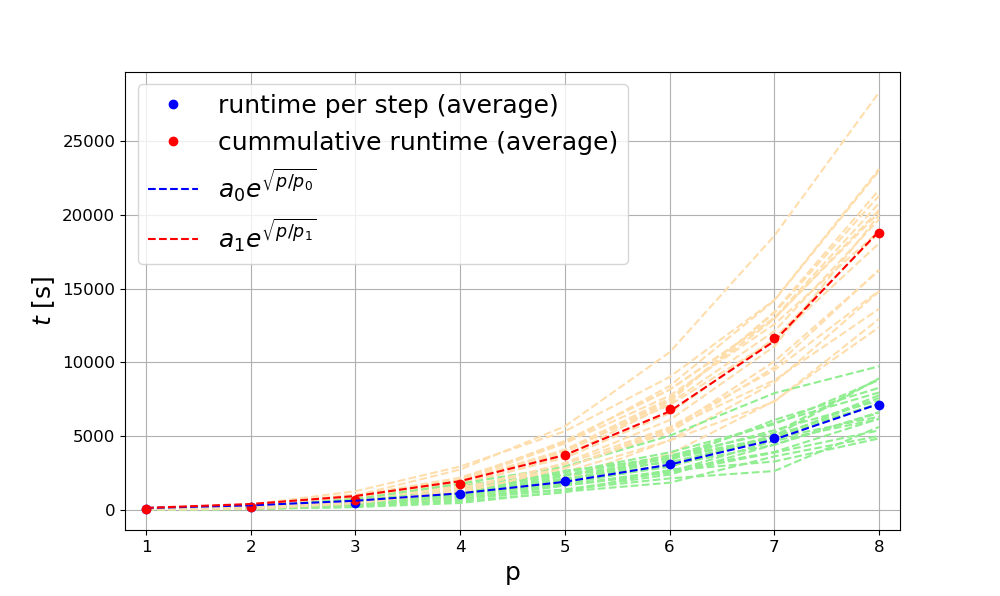
\includegraphics[width=0.6\textwidth]{figures/interp/runtime_15-nodal_ER050.png}
	\caption{Runtime (wall-clock time) when simulating the algorithm using the pyQuil INTERP method on 20 instances of ER graphs with 15 nodes and edge probability 0.5. The fit parameters for the runtime per step are $a_0 = 2.4 \pm 0.6$, $p_0 = 6.1 \pm 0.4$. The fit parameters for the cummulative runtime are $a_1 = 1.4\pm 0.2$ and $p_1 = 9.0\pm0.3$. The mean runtime per graph per step at $p=8$ is around 2700 seconds, or 45 minutes. A run for one graph starting from $p=1$ typically lasted 2 hours. The light green and navajo white dashed lines indicate the runtime per step and the cummulative time for one instance, respectively.}
\end{figure}

\begin{figure}[H]
	\centering
	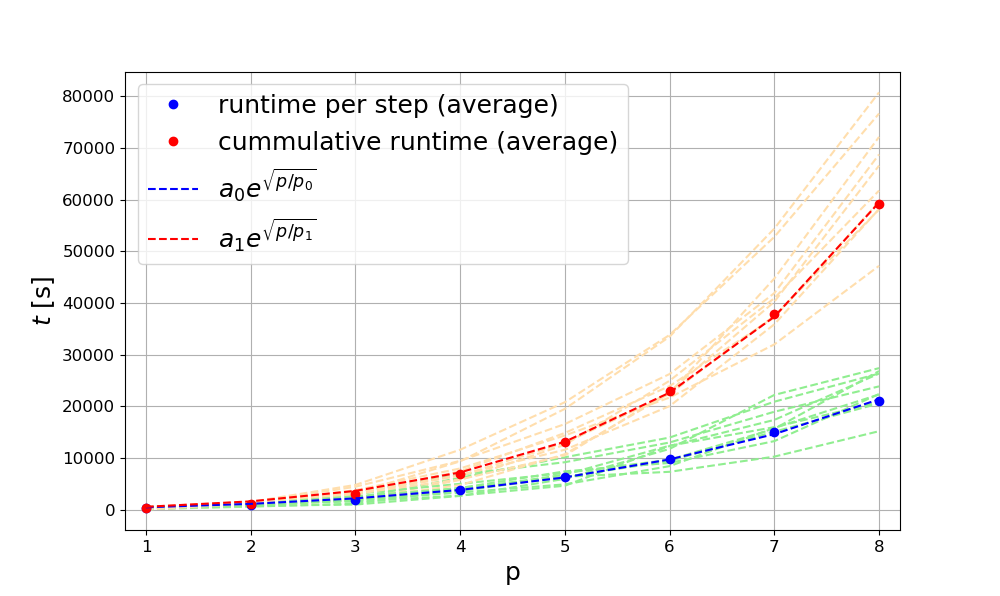
\includegraphics[width=0.6\textwidth]{figures/interp/runtime_15-nodal_ER075.png}
	\caption{Runtime (wall-clock time) when simulating the algorithm using the pyQuil INTERP method on 10 instances of weighted ER graphs with 15 nodes and edge probability 0.75. The fit parameters for the runtime per step are $a_0 = 60 \pm 7$, $p_0 = 4.3 \pm 0.2$. The fit parameters for the cummulative runtime are $a_1 = 44 \pm 5$ and $p_1 = 6.5\pm 0.2$. The light green and navajo white dashed lines indicate the runtime per step and the cummulative time for one instance, respectively.}
\end{figure}

\chapter{Fractional errors}
\label{appendix:fractional-error}

\begin{figure}[H]
	\centering
	\begin{subfigure}[t]{0.45\textwidth}
		\centering
		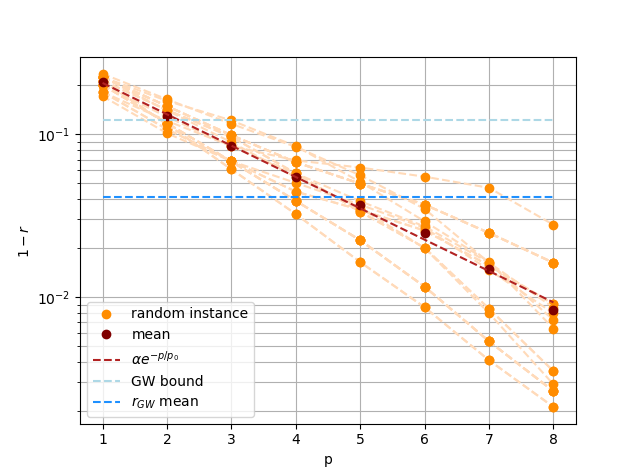
\includegraphics[width=\textwidth]{figures/interp/FOM_(unweighted)/EXP/FOM_3-regular-10-nodal_exp}
		\caption{10 nodes. Fit parameters $\alpha = 0.322 \pm 0.004$ and $p_0 = 2.26 \pm 0.03$.}
	\end{subfigure}
	~
	\begin{subfigure}[t]{0.45\textwidth}
		\centering
		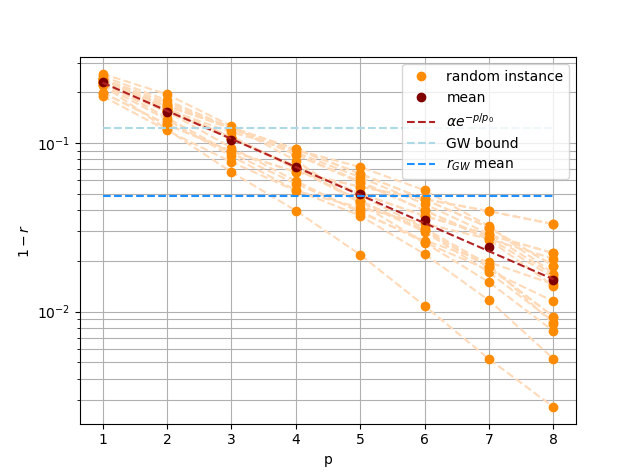
\includegraphics[width=\textwidth]{figures/interp/FOM_(unweighted)/EXP/FOM_3-regular-12-nodal_exp}
		\caption{12 nodes. Fit parameters $\alpha = 0.335 \pm 0.002$ and $p_0 = 2.61 \pm 0.02$.}
	\end{subfigure}
	\\
	\centering
	\begin{subfigure}[t]{0.45\textwidth}
		\centering
		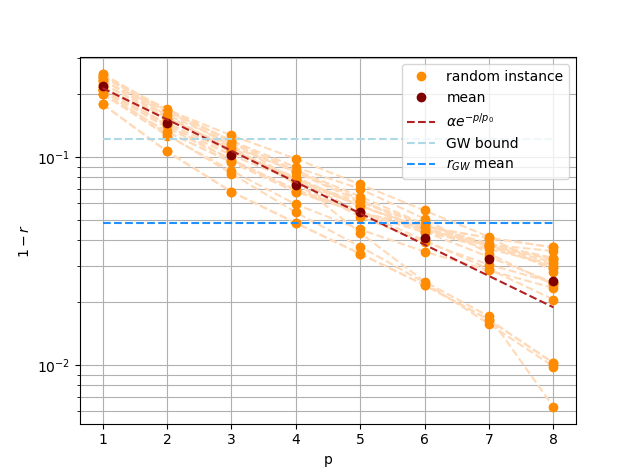
\includegraphics[width=\textwidth]{figures/interp/FOM_(unweighted)/EXP/FOM_3-regular-14-nodal_exp}
		\caption{14 nodes. Fit parameters $\alpha = 0.30 \pm 0.01$ and $p_0 = 2.9 \pm 0.1$.}
	\end{subfigure}
	~
	\begin{subfigure}[t]{0.45\textwidth}
		\centering
		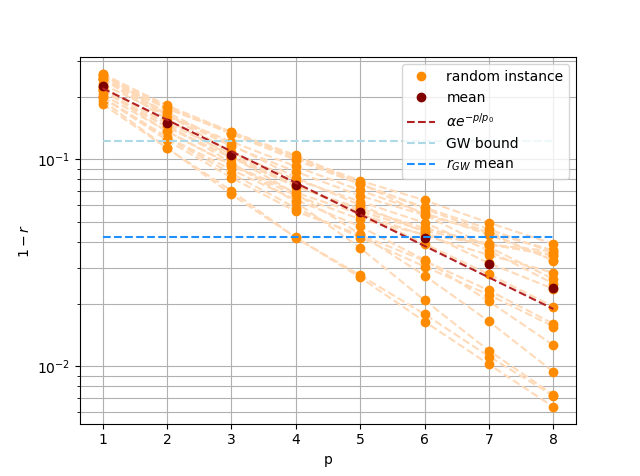
\includegraphics[width=\textwidth]{figures/interp/FOM_(unweighted)/EXP/FOM_3-regular-16-nodal_exp}
		\caption{16 nodes. Fit parameters $\alpha = 0.313 \pm 0.009$ and $p_0 = 2.9 \pm 0.1$.}
	\end{subfigure}
	\caption{The fractional error as a function of $p$ for unweighted 3-regular graphs using INTERP. For each $n$ 20 randomly generated instances were considered. A fit of the mean of the fractional error of those instances is included with model function $\alpha e^{-p/p_0}$ which suggests that the fractional error decays exponentially with $p$.}
\end{figure}

\begin{figure}[H]
	\centering
	\begin{subfigure}[t]{0.45\textwidth}
		\centering
		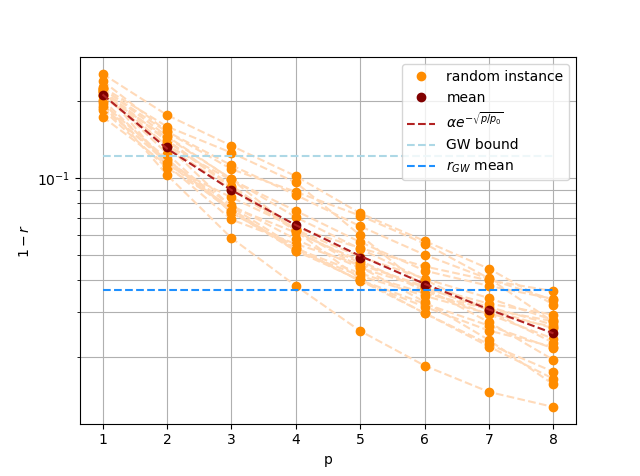
\includegraphics[width=\textwidth]{figures/interp/FOM_(weighted)/SQR/FOM_3-regular-10-nodal_sqr}
		\caption{10 nodes. Fit parameters $\alpha = 0.688 \pm 0.006$ and $p_0 = 0.723 \pm 0.008$.}
	\end{subfigure}
	~
	\begin{subfigure}[t]{0.45\textwidth}
		\centering
		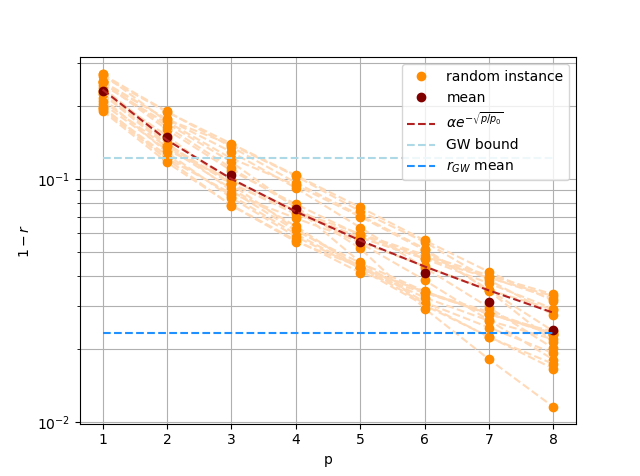
\includegraphics[width=\textwidth]{figures/interp/FOM_(weighted)/SQR/FOM_3-regular-12-nodal_sqr}
		\caption{12 nodes. Fit parameters $\alpha = 0.740 \pm 0.03$ and $p_0 = 0.75 \pm 0.04$.}
	\end{subfigure}
	\\
	\centering
	\begin{subfigure}[t]{0.45\textwidth}
		\centering
		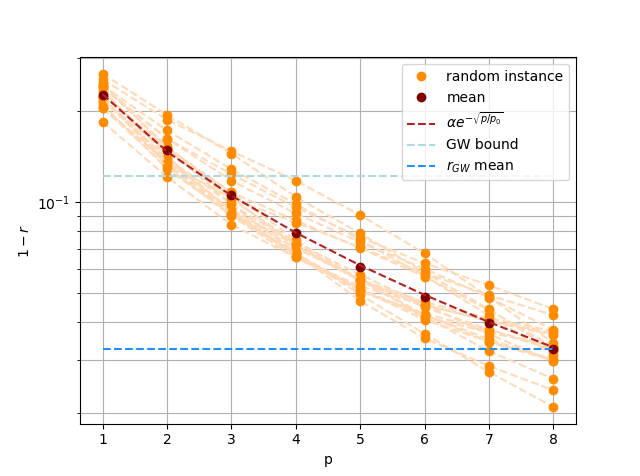
\includegraphics[width=\textwidth]{figures/interp/FOM_(weighted)/SQR/FOM_3-regular-14-nodal_sqr}
		\caption{14 nodes. Fit parameters $\alpha = 0.654 \pm 0.006$ and $p_0 = 0.90 \pm 0.01$.}
	\end{subfigure}
	~
	\begin{subfigure}[t]{0.45\textwidth}
		\centering
		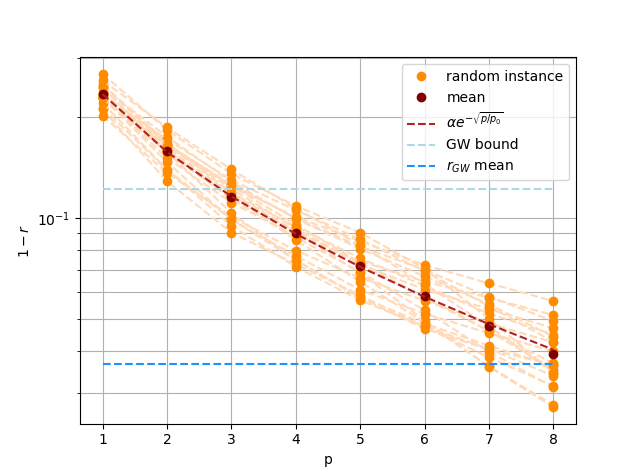
\includegraphics[width=\textwidth]{figures/interp/FOM_(weighted)/SQR/FOM_3-regular-16-nodal_sqr}
		\caption{16 nodes. Fit parameters $\alpha = 0.615 \pm 0.005$ and $p_0 = 1.08 \pm 0.01$.}
	\end{subfigure}
	\caption{The fractional error as a function of $p$ for weighted 3-regular graphs using INTERP. For each $n$ 20 randomly generated instances were considered. A fit of the mean of the fractional error of those instances is included with model function $\alpha e^{-\sqrt{p/p_0}}$ which suggests that the fractional error decays exponentially with the square root of $p$.}
\end{figure}

\begin{figure}[H]
	\centering
	\begin{subfigure}[t]{0.45\textwidth}
		\centering
		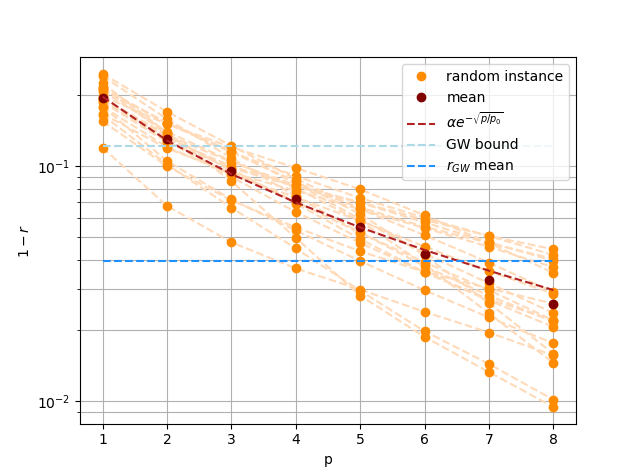
\includegraphics[width=\textwidth]{figures/interp/fom_er050_n11}
		\caption{11 nodes. Fit parameters $\alpha = 0.55 \pm 0.02$ and $p_0 = 0.93 \pm 0.04$.}
	\end{subfigure}
	~
	\begin{subfigure}[t]{0.45\textwidth}
		\centering
		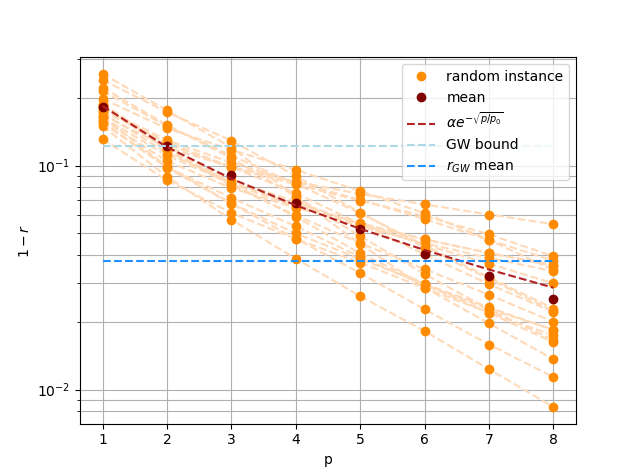
\includegraphics[width=\textwidth]{figures/interp/fom_er050_n12}
		\caption{12 nodes. Fit parameters $\alpha = 0.51 \pm 0.01$ and $p_0 = 0.96 \pm 0.04$.}
	\end{subfigure}
	\\
	\centering
	\begin{subfigure}[t]{0.45\textwidth}
		\centering
		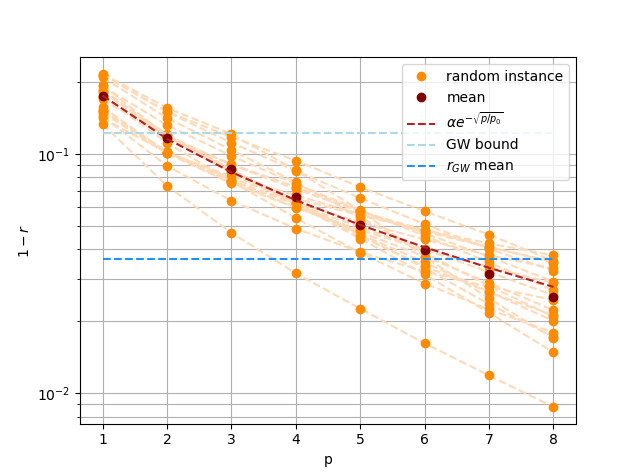
\includegraphics[width=\textwidth]{figures/interp/fom_er050_n13}
		\caption{13 nodes. Fit parameters $\alpha = 0.48 \pm 0.01$ and $p_0 = 0.99 \pm 0.03$.}
	\end{subfigure}
	~
	\begin{subfigure}[t]{0.45\textwidth}
		\centering
		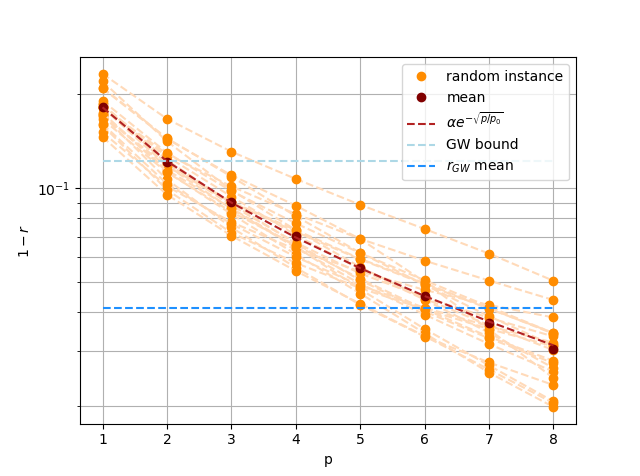
\includegraphics[width=\textwidth]{figures/interp/fom_er050_n14}
		\caption{14 nodes. Fit parameters $\alpha = 0.474 \pm 0.004$ and $p_0 = 1.09 \pm 0.01$.}
	\end{subfigure}
	\\
	\begin{subfigure}[t]{0.45\textwidth}
		\centering
		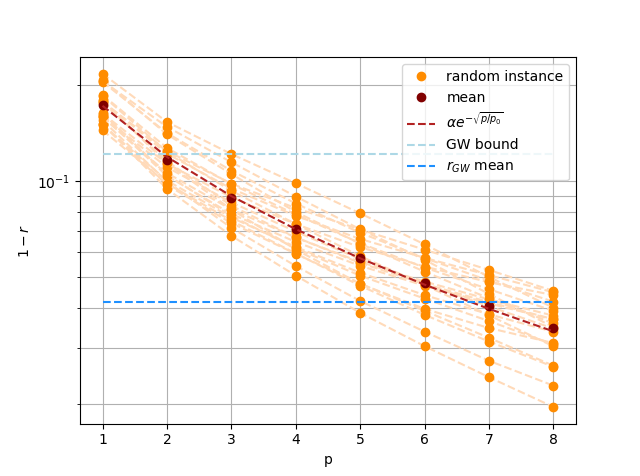
\includegraphics[width=\textwidth]{figures/interp/fom_er050_n15}
		\caption{15 nodes. Fit parameters $\alpha = 0.420 \pm 0.006$ and $p_0 = 1.26 \pm 0.03$.}
	\end{subfigure}
	\caption{The fractional error as a function of $p$ for ER-0.5 graphs using INTERP. For each $n$ 20 randomly generated instances were considered. A fit of the mean of the fractional error of those instances is included with model function $\alpha e^{-\sqrt{p/p_0}}$ which suggests that the fractional error decays exponentially with the square root of $p$. }
\end{figure}

\begin{figure}[H]
	\centering
	\begin{subfigure}[t]{0.45\textwidth}
		\centering
		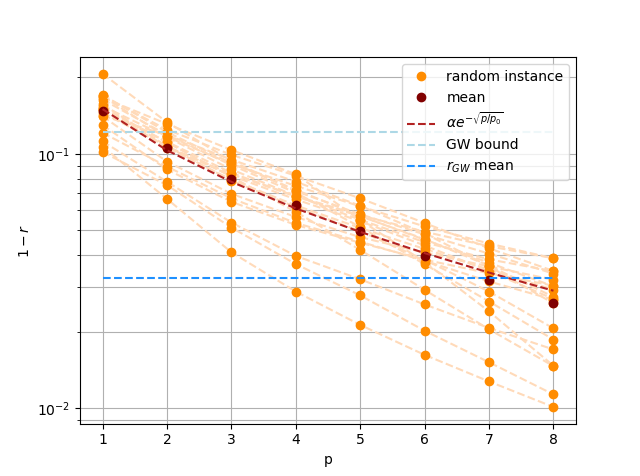
\includegraphics[width=\textwidth]{figures/interp/fom_er075_n11}
		\caption{11 nodes. Fit parameters $\alpha = 0.37 \pm 0.01$ and $p_0 = 1.24 \pm 0.06$.}
	\end{subfigure}
	~
	\begin{subfigure}[t]{0.45\textwidth}
		\centering
		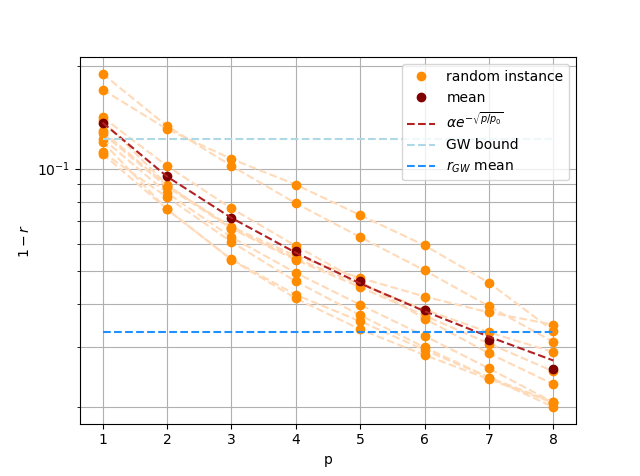
\includegraphics[width=\textwidth]{figures/interp/fom_er075_n12}
		\caption{12 nodes. Fit parameters $\alpha = 0.312 \pm 0.002$ and $p_0 = 1.4 \pm 0.02$.}
	\end{subfigure}
	\\
	\centering
	\begin{subfigure}[t]{0.45\textwidth}
		\centering
		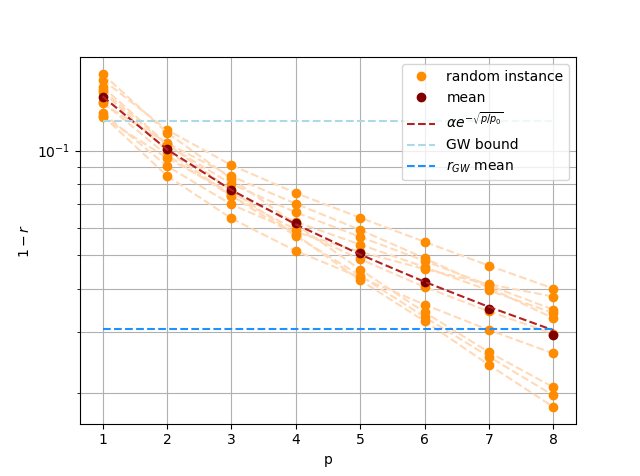
\includegraphics[width=\textwidth]{figures/interp/fom_er075_n13}
		\caption{13 nodes. Fit parameters $\alpha = 0.317 \pm 0.002$ and $p_0 = 1.42 \pm 0.01$.}
	\end{subfigure}
	~
	\begin{subfigure}[t]{0.45\textwidth}
		\centering
		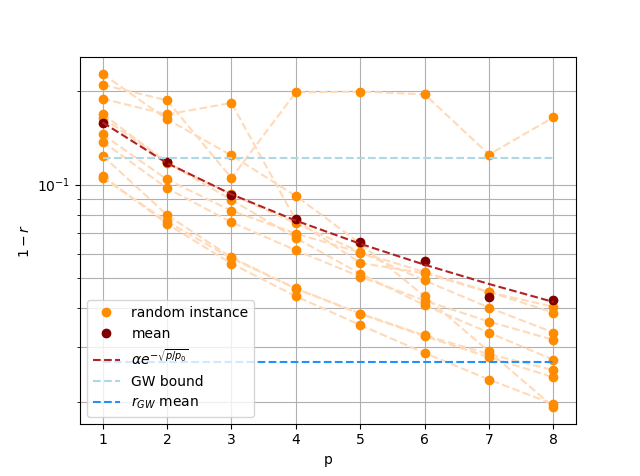
\includegraphics[width=\textwidth]{figures/interp/fom_er075_n14}
		\caption{14 nodes. Fit parameters $\alpha = 0.327 \pm 0.008$ and $p_0 = 1.89 \pm 0.08$. There seems to be an anomalous results in one of the 14 nodal graphs.}
	\end{subfigure}
	\\
	\begin{subfigure}[t]{0.45\textwidth}
		\centering
		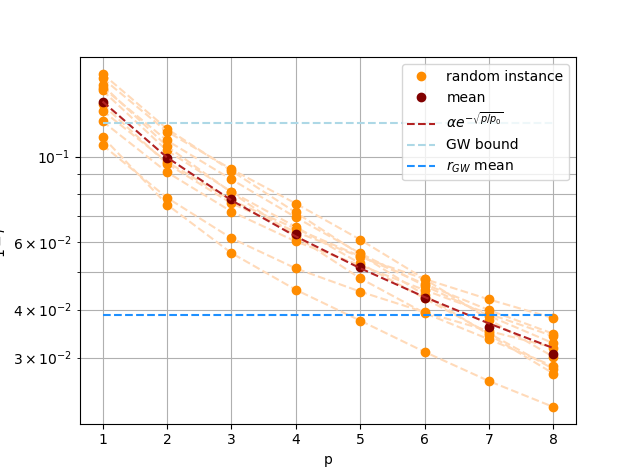
\includegraphics[width=\textwidth]{figures/interp/fom_er075_n15}
		\caption{14 nodes. Fit parameters $\alpha = 0.312 \pm 0.003$ and $p_0 = 1.53 \pm 0.02$.}
	\end{subfigure}
	\caption{The fractional error as a function of $p$ for ER-0.75 graphs using INTERP. For each $n$ 10 randomly generated instances were considered. A fit of the mean of the fractional error of those instances is included with model function $\alpha e^{-\sqrt{p/p_0}}$ which suggests that the fractional error decays exponentially with the square root of $p$. }
\end{figure}

\chapter{Software and Python packages}
\label{appendix:packages}

Python version 3.7.7 was used throughout this work. A list of the Python used packages and the corresponding versions is included in Table \ref{table:packages} 
\begin{table}[h!]
	\centering
	\begin{tabular}{||c  c||} 
		\hline
		Package & Version \\ [0.5ex] 
		\hline\hline
		cvxpy & 1.1.1 \\
		cvxgraphalgs & 0.1.2 \\
		matplotlib & 3.1.3 \\ 
		numpy & 1.18.5 \\
		pandas & 1.0.3 \\
		pyquil & 2.19.0 \\
		quantum-grove & 1.7.0 \\
		networkx & 0.3.4 \\
		scipy & 1.4.1 \\ [1ex] 
		\hline
	\end{tabular}
	\caption{Versions of relevant Python packages used for implementation.}
	\label{table:packages}
\end{table}

Moreover, the Rigetti Forest Software Development Kit (SDK) was used, which includes pyQuil, the Rigetti Quil Compiler (quilc), and the Quantum Virtual Machine (qvm). Forest SDK version 2.0 was used for this thesis.
